% Metódy inžinierskej práce

\documentclass[10pt,twoside,slovak,a4paper]{article}

\usepackage[slovak]{babel}
%\usepackage[T1]{fontenc}
\usepackage[IL2]{fontenc} % lepšia sadzba písmena Ľ než v T1
\usepackage[utf8]{inputenc}
\usepackage{graphicx}
\usepackage{url} % príkaz \url na formátovanie URL
\usepackage{hyperref} % odkazy v texte budú aktívne (pri niektorých triedach dokumentov spôsobuje posun textu)

\usepackage{cite}
\usepackage{times}

\pagestyle{headings}

\title{Použitie hier a VR pri rehabilitácii\thanks{Semestrálny projekt v predmete Metódy inžinierskej práce, ak. rok 2022/23, vedenie: Ing. Igor Stupavský}} % meno a priezvisko vyučujúceho na cvičeniach

\author{Pavol Čížik\\[2pt]
	{\small Slovenská technická univerzita v Bratislave}\\
	{\small Fakulta informatiky a informačných technológií}\\
	{\small \texttt{xcizik@stuba.sk}}
	}

\date{\small 30. september 2022} 



\begin{document}

\maketitle

\begin{abstract}
Vo svojom článku by som sa chcel venovať téme použitie virtuálnej realita a gamifikácie pri rehabilitáciach. Takéto rehabilitácie by sa mohli použiť po zlomeninách alebo u pacientov po mŕtvici. Pretože medzi následky mŕtvice patrí nemožnosť normálnych kontrolovaných pohybov a problémy s hmatom a jemnou motorikou. 

V článku by som sa chcel zamerať na výhody a nevýhody, ktoré by takáto liečba priniesla. Pozrieť sa na ceny virtuálnych realít. A či by bolo možné rehabilitovať aj doma. 

Hry a virtuálna realita by mohli pacientov viacej motivovať do cvičenie čo by mohlo mať za dôsledok rýchlejšie zotavenie. Preto si myslím že táto téma má veľký význam a v budúcnosti by mohli hry a virtuálna realita výrazne pomôcť pri rehabilitáciach.
\end{abstract}



\section{Úvod}

V posledných rokoch sa poožitie VR a hier rozšírilo do mnohých oblastí života. V článku sa zameriavam presnejšie na použitie v zdravotníctve. Specifickejšie použitie hier a VR pri rehabilitáciach, či už u pacientov po mŕtvici ale aj pri bežných úrazoch. 

Napríklad sa zameriavam na VR nástroj Leap motion. Ďalším nástrojom použitím v medicíne je  SilverTune. Ktorá pomáha pacientom po mŕtvici. V článku sa zameriavam ale aj na iné nástroje ktoré sú použité napríklad aj pri rehabilitácii členku. 

Samozrejme všetko má svoje výhody ale aj nevýhody preto sú v článku zhrnuté aj výhody a nevýhody, ktoré použitie týchto zariadení so sebou prináša.

\newpage

\section{Použitie v praxi}


\subsection{SilverTune}
SilverTune je nástroj, ktorý je výsledkom výskumu, ktorého hlavným cielom bolo vytvoriť multi-senzorový hudobný nástroj. Výskum sa zameriaval na použitie tohto nástorje pri rehabilitácií starších pacientov po mŕtvici v Singapure.

SilverTune je ako hudobný nástroj, ktorý poskytuje šesť typov hudobných zvukov a herných interakcií, aby uspokojil rôzne preferencie pacientov a terapeutické požiadavky na pohyb. 

SilverTune môže tiež zaznamenávať údaje, analyzovať výkon v reálnom čase a poskytovať spätnú väzbu pacientom aj terapeutom.

Mobilná aplikácia SilverTune bola vyvinutá ako sprievodná pre muzikoterapiu SilverTune. Aplikácia zaznamenáva profil používateľa a údaje zadané zo SilverTune pre budúcu analýzu terapeutom. 

Na hranie pomocou zariadenia SilverTune boli vyvinuté dve hry. Prvou je dostihová hra, v ktorej sa kôň pohybuje po dostihovej dráhe. Druhou je stolnotenisová hra\ref{fig:SilverTune Stolný tennis}, v ktorej sa loptička na stolný tenis musí podávať cez sieť, aby získala body. Dostihová hra uľahčovala ohýbanie a predlžovanie ramien, zatiaľ čo stolnotenisová hra uľahčovala horizontálny únos a addukciu ramena.\cite{9483850}

\begin{figure}[ht]
    \centering
    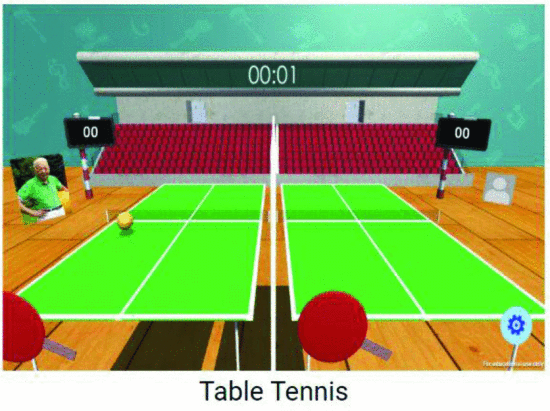
\includegraphics[width = 0.5\textwidth]{obrazky/table_tennnis.png}
    \caption{Stolný tennis}
    \label{fig:SilverTune Stolný tennis}
\end{figure}


\subsection{Leap motion}
Leap motion dostal veľa pozornosti in posledných pár rokoch z dôvodu jeho nemeratelného množstva použití ako napríklad robotika, vzdelávanie, medicína atď. Hlavnou myšlienkou gamifikácie rehabilitácie je pomôcť rozvíjať svalový tonus, zefektívniť rehabilitáciu a motivovať pacientov.

Ukázalo sa, že VR a hry sú prospešné pri zlepšovaní funkcie horných končatín, ak sa používajú ako doplnok k bežnej starostlivosti alebo v porovnaní s konvenčnou terapiou.

Hra bola vyvinutá  pomocou Unity 3D a volá sa Escape game\ref{fig:LeapMotion escape game}. Hra má rôzne možnosti, úlohy a cvičenia súvisiace s 3D chytaním, ukazovaním, zdvíhaním, hádzaním a ďalšími cvičeniami na rehabilitáciu rúk. Hlavnou súčasťou tejto VR rehabilitácie je Leap Motion, ktorý sleduje ruky. 

Všetky predmety a štruktúry hry boli vytvorené v Autodesk 3D Max a Cinema 4D, potom importované do prostredia Unity.\cite{7926560}

\begin{figure}
    \centering
    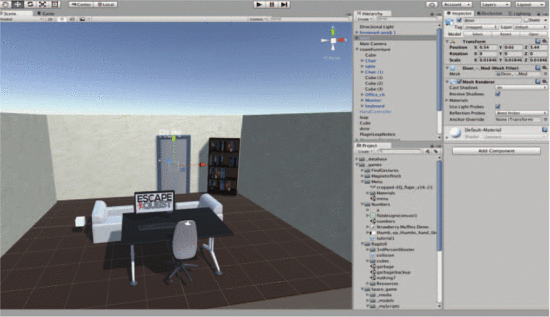
\includegraphics[width = 0.5\textwidth]{obrazky/Escape game.png}
    \caption{Escape game}
    \label{fig:LeapMotion escape game}
\end{figure}

\subsection{Myo armband}
Systém na rehabilitácie rúk, inšpirovaný videohernými zariadeniami. Tento systém sa skladá z Myo band a robotickej rukavice. Myo band je nositeľné zariadenie v hodnote ~200 eur.

Zariadenie poskytuje dva druhy údajov, priestorové a gestové. 
Priestorové údaje informujú o orientácii a pohybe ramena používateľa, zatiaľ čo gestové údaje informujú o tom, čo používateľ robí rukou. Všetky údaje sa komunikujú cez Bluetooth s Unity3D. Tatktiež sú použité dotykové ploch  na detekciu úplne otvorenej/zatvorenej ruky.

V Unity 3D bola vytvorená hra na tréning ruky, v ktorej musí používateľ chytiť, držať a prepravovaťa kocku v niekoľkých čoraz náročnejších úrovniach. V hre hráč vidí virtuálne ruky/ramená, ktoré replikujú pohyby používateľa, vďaka tomu sa použvateľ cíti viacej ponorený do hry. 

V súčasnosti hra funguje nasledovne: používateľ nosí Myo band na zdravom predlaktí a vykonáva požadované pohyby\ref{fig:Myoband pohyby}, ktoré sa premietajú do pohybu virtuálnej ruky.
Pohyby rúk sa potom replikujú  do pohybu robotickej rukavice, ktorú používateľ nosí na rehabilitovanej ruke. 
 
Systém bol doteraz testovaný iba na zdravých jedincoch, ale plánujú sa aj testy s pacientami po mozgovej príhode. Preto je tažké jednoznačne povedať či je tento spôsob rehabilitácie účinný a  sú stále potrebné daľšie testy a štúdie na preukázanie benifitov pre pacientov\cite{7088817}

\begin{figure}
    \centering
    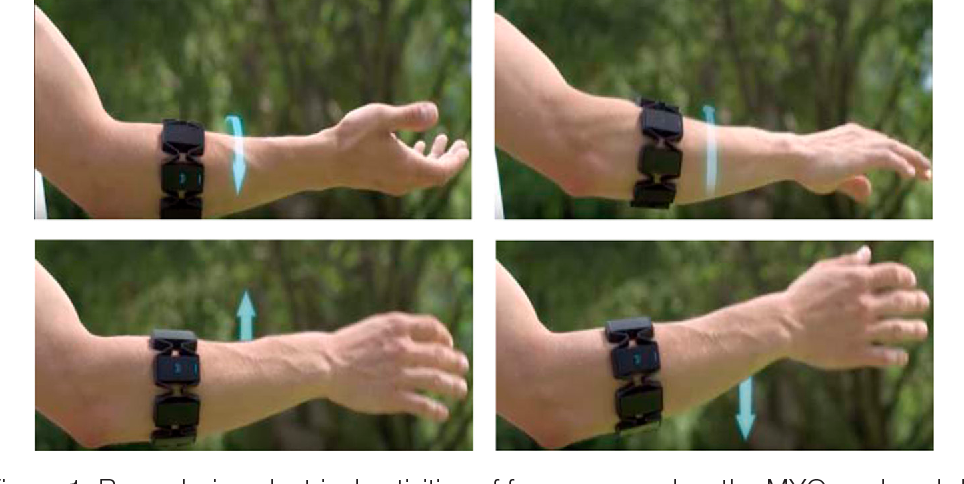
\includegraphics[width = 0.5\textwidth]{obrazky/Myoband.png}
    \caption{Myoband}
    \label{fig:Myoband pohyby}
\end{figure}

\subsection{PhyRe}\cite{9564051}

\section{Výhody} 
Jednou z hlavných výhod VR reality a hier bolo hlavne počas pandémie COVID-19, že rehabilitácie vedeli prebiehať na dialku.



\section{Nevýhody}
..........\cite{7523762}


\section{Možné problémy}
......

\section{Reakcia na témy z prednášok}
\paragraph{1}

.......
\paragraph{2}


.......
\paragraph{3}

.......



\section{Záver} 
..........






\bibliography{literatura}
\bibliographystyle{plain} % prípadne alpha, abbrv alebo hociktorý iný
\end{document}
